\documentclass[border=4pt]{standalone}
% Preámbulo común de las figuras. Cada figura es un documento standalone
% que se compila a SVG con scripts/build_figures.sh
\usepackage[utf8]{inputenc}
\usepackage{amsmath}
\usepackage{tikz}
\usepackage[american, siunitx]{circuitikz}
\usetikzlibrary{arrows.meta,calc,decorations.pathmorphing,patterns}
\tikzset{
  >={Stealth[length=2.2mm]},
  eje/.style={->, thin},
  hilo/.style={thick},
}
% Paleta común: tonos medios legibles sobre fondo claro
\definecolor{azul}{RGB}{31,94,168}
\definecolor{rojo}{RGB}{192,57,43}
\definecolor{verde}{RGB}{39,128,73}
\definecolor{naranja}{RGB}{211,120,30}
\definecolor{morado}{RGB}{125,60,152}

\begin{document}
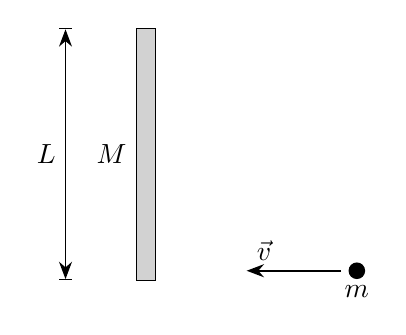
\begin{tikzpicture}[scale=1.0]
  \fill[gray!35] (0,0) rectangle (0.24,3.2);
  \draw (0,0) rectangle (0.24,3.2);
  \node[left] at (0,1.6) {$M$};
  \draw[|<->|] (-0.9,0) -- node[left]{$L$} (-0.9,3.2);
  \fill (2.8,0.12) circle (3pt) node[below=2pt]{$m$};
  \draw[->, thick] (2.6,0.12) -- (1.4,0.12) node[above right]{$\vec{v}$};
\end{tikzpicture}
\end{document}
